% Chapter 3

\chapter{Tecnologías y herramientas en el reconocimiento de iris} % Main chapter title

\label{Capítulo 3} % For referencing the chapter elsewhere, use \ref{Chapter3} 

%----------------------------------------------------------------------------------------

% Define some commands to keep the formatting separated from the content 
%\newcommand{\keyword}[1]{\textbf{#1}}
%\newcommand{\tabhead}[1]{\textbf{#1}}
%\newcommand{\code}[1]{\texttt{#1}}
%\newcommand{\file}[1]{\texttt{\bfseries#1}}
%\newcommand{\option}[1]{\texttt{\itshape#1}}

%----------------------------------------------------------------------------------------

\section{Introducción}

Conocido ya el comportamiento general de los sistemas de reconocimiento de personas y de manera mas específica los basados a través del iris que se ejecutan en condiciones no ideales, en este capítulo vamos a estudiar las herramientas y tecnologías existentes en las que nos apoyaremos para desarrollar un nuevo método de extracción de características que sea integrado en un sistema de reconocimiento de este tipo con el objetivo de evaluar su rendimiento con los obtenidos usando diferentes métodos de extracción de características. \\

Como bien hemos podido ver en el capítulo anterior, un sistema de reconocimento biométrico se compone de cuatro elementos principales: la adquisición de imágenes, el pre-procesamiento, la extracción de características y la comparación de las mismas. Aunque el propósito de este Trabajo Fin de Master es el de diseñar e implementar un nuevo método de extracción de características, también será necesario desarrollar el resto de componentes que forman un sistema de reconocimiento biométrico para evaluar los resultados, haciendo uso para ello de las herramientas que se describen en este apartado.\\ 

Para el desarrollo de la etapa de adquisición de imágenes haremos uso de la base de datos \textbf{CASIA V4} \footnote{Disponible en el sitio web de CASIA (http://biometrics.idealtest.org)}, la cual contiene un conjunto de imágenes tomadas a individuos de los ojos izquierdo y derecho afectadas por diferentes factores de calidad, mientras el resto de las etapas se fundamentarán en diferentes librerías. Mediante la librería \textbf{USITv1.0.3} \footnote{Disponible en el sitio web de USIT (http://www.wavelab.at/sources/USIT/)}, la cual se basa en \textbf{OpenCV} \footnote{Disponible en el sitio web de OpenCV (http://opencv.org)} y \textbf{Boost} \footnote{Disponible en el sitio web de Boost (http://www.boost.org)} se desarrollarán las etapas de pre-procesamiento y comparación de características. Del mismo modo, la etapa de extracción de caracterísitcas se basará en el framework de desarrollo \textbf{LIP-VIREO} \footnote{Disponible en el sitio web de LIP-VIREO (https://code.google.com/archive/p/lip-vireo/)}. De la misma, se hará uso de los diferentes métodos de extracción de características que expone y que serán los que se comparen con el método propuesto en este Trabajo Fin de Master. \\

El desarrollo del método de extracción de características sobre el que se basa esta memoria se apoyará en la librería \textbf{LIP-VIREO}. \\



%----------------------------------------------------------------------------------------

\section{OpenCV}

OpenCV (Open Source Computer Vision Library) es una librería de código abierto lanzada bajo licencia BSD y de uso libre académico y comercial. Esta implementada para C++, C, Python y Java, además de tener soporte para múltiples plataformas como Windows, Linux, Mac OS, iOS y Android. Está diseñada para aplicaciones en tiempo real así como para proporcionar un entorno de desarrollo fácil de utilizar y altamente eficiente. \\

Fue desarrollada inicialmente por Intel para el uso en visión artificial, apareciendo su primera versión en 1999. Se centra en funcionalidades que abarcan una gran gama de áreas en el proceso de visión como reconocimiento de objetos, calibración de cámaras, visión estérea y visión robótica. Su alta influencia en el campo de la visión por computador ha echo que sea base fundamental en el tratamiento digital de imágenes. \\

La versión 3.2.0 es la última versión que dispone esta libería, y sobre la que se basará el nuevo método de extracción de características. También forma parte del núcleo de la librería \textbf{USIT}.

%----------------------------------------------------------------------------------------

\section{Boost}

Boost es un conjunto de librerías multiplataforma de software libre diseñada para extender las capacidades del lenguaje de programación C++. Al igual que la librería \textbf{OpenCV} su licencia es de tipo BSD, lo que permite que pueda ser utilizada en cualquier tipo de proyeto sean comerciales o no. \\

El uso de esta libreria en su versión 1.63.0 será necesario para el desarrollo del nuevo método de extracción de características en conjunto con la librería \textbf{OpenCV}, que al igual que esta forma también parte del núcleo de la librería \textbf{USIT}. \\


%----------------------------------------------------------------------------------------

\section{USIT}

USIT (University of Salzburg Iris Toolkit v2) es un paquete software desarrollado por la Universisdad de Salzburgo empleado en el reconocimiento del iris y lanzado para plataformas Windows y Linux. Este paquete software incluye algoritmos para realizar tareas de pre-procesamiento de iris, extracción de características y comparación de caracaterísticas. USIT está basado en una fácil y simple herramienta manejada por línea de comandos \cite{Reference18} \cite{Reference19}.

Se utilizarán los métodos y algoritmos que este software ofrece en su versión v1.0.3 para desarrollar las etapas de pre-procesamiento y comparación del sistema de reconocimiento, así como también se utilizarán los métodos de extracción de características mediante los cuales se podrá medir el nivel de eficiencia y fiabilidad del método propuesto. \\

Como se vió en el capítulo anterior, la etapa de pre-procesamiento en el reconocimiento del iris en condiciones no ideales se compone a su vez de otra serie de tareas como son la detección de falsedad para evitar falsos reclamos como una imagen impresa del iris o una grabación del mismo, a través de técnicas de medición de indicadores de espécimen vivo. La evaluación de calidad para la detección y corrección de factores como el emborronado por desenfoque y la dilatación de pupila es otra de las tareas dentro de la etapa del preprocesamiento, así como la segmentación del iris una vez localizado. Es en esta última fase donde la librería USIT aporta dos algoritmos, “caht” y “wahet”. Estos algoritmos usan modelos geométricos a través de círculos y elipses para representar las partes del limbus (anillo limbal) y la pupila del ojo humano. \\

El algoritmo \textbf{Caht} emplea un modelo circular para el limbus y la pupila, que son los límites externos e internos del iris. Esta basado en los métodos de la transformada circular de Hough y la mejora de contraste. La transformada de Hough es una técnica utilizada para la detección de figuras en imágenes digitales que realiza un proceso mediante el cual se divide la imagen en regiones y objetos cuyos píxeles poseen atributos similares. Principalmente es una técnica para detectar líneas rectas en imágenes, aunque también sirve para la detección de curvas, siendo muy robusta frente al ruido y la existencia de huecos en la frontera.  Aprovechando las cualidades de dicha técnica, este algoritmo aplica una transformada circular para la detección de los bordes internos y externos del iris \cite{Reference18}. \\

\textbf{Wahet}  propone un algoritmo basado en dos etapas para la localización y mapeo de la textura del iris dentro de las coordenadas polares de Daugman. En esta solución la detección del centro y la localización del límite del iris se desacoplan al contrario de lo que sucedía en los algoritmos con un enfoque mas tradicional, siendo por tanto el espacio de búsqueda para cada estado reducido. Este algoritmo utiliza un modelo elíptico a diferencia del modelo circular del algoritmo anterior, pero si comparte el uso de la transformada de Hough aunque emplea una adaptación multiescala de la misma para estimar la posición aproximada del centro del iris y una transformada elipsopolar de Hough para encontrar el segundo límite basado en la salida del primero \cite{Reference18}. \\

Ambos algoritmos de segmentación dan como resultado una matriz de valores de intensidades de gris cada uno con la misma dimensión por cada imagen, es en esta estructura donde se almacena la textura del iris localizado. Cabe recordar que el iris segmentado presenta afecciones producidas por factores de calidad como la oclusión de pestañas y párpados. \\

Del mismo modo, el paquete USIT proporciona una serie de métodos para realizar la etapa de comparación de características una vez estas han sido extraídas. Existen dos tipos de comparadores, entre los que están los basados en los algoritmos de extracción de características, es decir, esos comparadores de característiacs sólo son utilizados para los datos que ha sido obtenidos a través de su respectivo método de extracción de características. En este sentido, la librería USIT proporciona los métodos comparadores \textit{koc} para el algoritmo de extracción de características \textit{Ko}, \textit{cbc} para el método \textit{cb}, \textit{dctc} para el método \textit{dct}, \textit{lbp} para el método \textit{lbpc}, \textit{siftc} para el método \textit{sift} y \textit{surfc} para el método \textit{surf}. El otro tipo de comparador que ofrece USIT es en un ámbito más general y está basado en la distancia de Hamming, este método es aplicado al resto de los métodos de extracción de características. \\

La extracción de características es la etapa que más interés despierta y la que mayor tiempo de investigación ha necesitado en el reconocimiento del iris. Actualmente existen múltiples algoritmos y métodos para extraer las características principales de una imagen, siendo hoy día un campo en el que se continúa investigando para conseguir mejorar en lo ya existente y ajustar aun mas la selección de dichas características. Esta etapa permite un amplio abanico de soluciones y propuestas como se puede observar en las que ofrece la librería USIT, siendo la fase de la misma la que más algoritmos propone como posibles soluciones.\\

Cada uno de los algoritmos presentados en la etapa de extracción de características por la librería USIT expone sus propias técnicas y métodos basados en mejoras de soluciones ya existentes algunos y en novedosas técnicas aplicadas a las matemáticas otros. Todos comparten en común el uso de las librerías OpenCV y Boost para su implementación. A continuación se hará un pequeña descripción del funcionamiento y finalidad de cada uno de los algoritmos \cite{Reference18} \cite{Reference19}. \\

El algoritmo Log Gabor trata la imagen como si fuese una señal a la que le analiza la frecuencia como hacen la mayoría de los filtros, pero en este caso los filtros Gabor permiten analizar simultáneamente las características de espacio y frecuencia, lo que significa que es posible determinar en que parte de la imagen se produce una determinada frecuencia. De este modo la frecuencia está localizada \cite{Reference18} \cite{Reference19}. \\

Al tratar las imágenes como una señal, se suele trabajar en el dominio de la frecuencia mediante la transformada de Fourier. En definitiva, los filtros de Gabor conforman un banco de filtros capaces de extraer información sobre las texturas de una imagen aprovechando la información sobre la distribución espacio-local de color o nivel de intensidades que esta provee. \\

De este modo los filtros aplicados a las texturas se pueden utilizar para realizar operaciones como la de realzar las variaciones de intensidad allí donde se producen y así poder detectar las características principales de la imagen. También se puede utilizar para suavizar la imagen reduciendo las variaciones de intensidad entre pixeles vecinos, eliminar ruido modificando aquellos pixeles cuyo nivel de intensidad sea muy diferente al de sus vecinos y detectar bordes en aquellos pixeles donde se produce un cambio brusco en la función intensidad. \\

Los filtros que se utilizan en este algoritmo son máscaras (matriz de coeficientes) que se aplican a la textura de la imagen para obtener el efecto deseado. El tipo de filtrado vendrá determinado por el tipo de la máscara. \\

Otro de los métodos que contiene la librería USIT es el implementado por el algoritmo QSW (Quadratic Spline Wavelet), el cual se basa en la idea básica de que la fuerte variación en puntos locales de la textura en la imagen del iris denotan la aparición o desaparición de una estructura de imagen importante, y por tanto son utilizados para representar las características principales del iris \cite{Reference18} \cite{Reference19}.\\

El procedimiento de extracción de características de este algoritmo incluye dos pasos; uno primero en el que se construye un conjunto de intensidades de una dimensión para caracterizar la información mas importante de la imagen original del iris en dos dimensiones, y un segundo paso en el que usando una clase wavelet, una secuencia de posiciones de puntos locales con fuertes variaciones en dichas señales de intensidades se registra como característica. Al igual que el algoritmo Log Gabor, se realiza una descomposición de la textura a señal de una dimensión, por la que la textura del iris es normalizada. \\

El siguiente algoritmo de la librería USIT corresponde al algoritmo KO. La tarea de extracción de características en este algoritmo se realiza aplicando un análisis de cambios basado en la suma acumulativa. Este método sugiere descartar partes de la textura del iris en forma de grados, de 45º a 315º para el lado derecho de la textura y de 135º a 225º del lado izquierdo \cite{Reference18} \cite{Reference19}. \\

El proceso que sigue este algoritmo para la extracción de características de la textura de un iris es el siguiente; una vez obtenida dicha textura se divide en regiones básicas de tamaño 8x3 pixeles, es decir, cada región se compondrá de 24 pixeles o celdas. Para cada una de esas regiones se calcula el valor medio de intensidades de escala de grises. Dichas regiones son agrupadas horizontal y verticalmente, siendo recomendable que los grupos estén compuestos por cinco regiones. Finalmente se calcula la suma acumulativa sobre cada grupo para generar un código del iris. Si las sumas acumulativas están en un pendiente creciente se codificará con un 1, si en caso contrario la pendiente es decreciente se codificará con un 2, para cualquier otro caso se asignará un 0 al código. \\

Con el fin de obtener un vector binario de características de la textura del iris, el código resultante del iris se reorganizará de tal modo que la primera mitad contenga todas las pendientes ascendentes y la segunda mitad todas las pendientes descendentes. \\

La mayoría de los algoritmos que propone esta librería se fundamentan en las teorías que Rathbeg empleó en la investigación y desarrollo de su tesis doctoral sobre la biometría a través del reconocimiento del iris. De echo, uno de los algoritmos que compone la librería USIT (el algoritmo CR) esta basado en el algoritmo estándar de Rathbeg, cuya base se encuentra en reducir el número de bits a comparar del código binario que representa la textura del iris. Trata de minimizar la información sobre un 5\% combinándola en los primeros bits, es decir, en los primeros bits del código del iris es donde se concentra la combinación de los mismos. De esta forma se consigue descartar de forma rápida y temprana los códigos que sean improbables de emparejar, evitando así el tener que comparar todos los bits de cada código del iris, lo que produciría un aumento en tiempo de cómputo incremental \cite{Reference18} \cite{Reference19}.\\

El algoritmo basado en el contexto (CB) es también empleado en como método en la librería USIT. Este algoritmo lo que hace es ir examinando la textura del iris en bloques de X x Y píxeles, donde el valor de cada uno de los píxeles de esos bloques es discreteado mapeando los valores de escala de grises de todos los píxeles incluidos (Pi) a un número natural inferior a un parámetro k predefinido, donde n es el número de posibles valores de escala de grises que se puede tomar. Una vez que todos los píxeles de la textura del iris son discretizados se calcula el valor medio de los píxeles contenidos en cada bloque, asignándole dicho valor al bloque como código del mismo. Finalmente, se genera un código de iris de dos dimensiones con respecto al número de filas obtenidas y concatenando los códigos resultado de todos los bloques de pixeles X x Y discretizados (Pi /n/k) \cite{Reference18} \cite{Reference19}. \\
 
Otro de los algoritmos que compone esta librería es el basado en la transformada  discreta del coseno. El algoritmo DCT (discrete cosine transform) es una variación de la transformada discreta de Fourier donde la imagen se descompone en suma de de cosenos. Este tipo de algoritmo es usado para la comprensión y reducción de datos, aunque el ámbito que se le da en la librería USIT es para la extracción de diferentes características de una imagen. Lo que hace el algoritmo DCT es comprimir toda la información de la imagen concentrándola en unos pocos coeficientes que se localizan en la esquina superior izquierda de la matriz de valores reales resultantes. La imagen que resulta de esta operación mostrará bajos valores o cero en los píxeles, exceptuando la esquina superior izquierda de la misma, donde las intensidades son mas altas. Estos coeficientes de baja frecuencia y alta intensidad que se sitúan en la esquina superior izquierda son los que llevan la mayoría de la información de la imagen original. Una vez que el algoritmo ha realizado el proceso de comprensión de la imagen y situado los coeficientes mas relevantes de la imagen, se suelen emplear dos métodos para la extracción de características en base a esos coeficientes obtenidos \cite{Reference18} \cite{Reference19}. \\

El primero de ellos emplea una técnica basada en ventanas cuadradas para extraer los coeficientes con menor frecuencia de la matriz resultante L x L = L2. Este método hace uso de que DCT pone la mayoría de la información de la señal en el componente dc y los componentes de menor frecuencia. Se van creando ventanas cuadradas desde el origen (0,0) de la matriz y se van obteniendo los coeficientes de dichas submatrices en orden descendente. El segundo método es una alternativa zig-zag donde los coeficientes se seleccionan dependiendo de su magnitud.\\

El último de los algoritmos de la etapa de extracción de características que provee la librería USIT fusiona las modalidades biométricas de iris y cara.  El algoritmo GFCF (Gaussian Face and Face-part Classifier Fusion) se basa en el reconocimiento del iris con una separación previa en conjuntos de buena calidad, por lo que debe realizar previamente una detección robusta y eficiente de los ojos en la cara. Este algoritmo combina múltiples y diferentes propuestas de detección de objetos para resolver la detección de caras en ambientes heterogéneos y la localización del ojo antes de la segmentación. Fusiona detectores de objetos arbitrariamente que realizan la tarea de extracción de características calculando propiedades de regiones de la imagen, seleccionando características discriminatorias que se evalúan con respecto al objeto a ser detectado y clasificando juzgando si una ventana data representa al objeto en si o no \cite{Reference18} \cite{Reference19}. \\



%----------------------------------------------------------------------------------------

\section{CASIA-Iris}

A pesar de contar con un patrón para el reconocimiento de personas que posee unas características muy precisas e ideales debido al origen de su naturaleza como es el iris, son muchas las tareas y desafíos que se presentan y quedan pendientes en el desarrollo de un algoritmo de alta calidad para conseguir una alta tasa de efectividad. Hay que tener en cuenta que el reconocimiento automático del iris tiene que hacer frente a múltiples y diversas variaciones impredecibles de las imágenes del iris que se pueden dar en aplicaciones del mundo real. Por ello, pueden producirse situaciones en las que se deba reconocer imágenes de iris con una pobre calidad, con posibles deformaciones, imágenes de iris que se han tomadas a distancia o en movimiento, incluso imágenes de iris falsas que se encuentran impresas en un papel o través de una fotografía. Por todo esto, se diseñó y desarrolló una rápida solución para solventar estos problemas, creando una base de datos de imágenes de iris que incluyesen todas esas variaciones. \\

Con esta idea nació la base de datos CASIA Iris Image, desarrollada por un grupo investigación del instituto “Chinese Academy of Sciences - Institute of Automation (CASIA), China” y liberada para la comunidad internacional de biometría, la cual se ha ido actualizando desde su primera versión CASIA-IrisV1. Las imágenes de la base de datos CASIA-Iris contiene imágenes de mas de 3.000 usuarios de 70 países diferentes, lo que hace que exista una alta diversidad de rasgos y características. \\

CASIA-IrisV4 es una extensión de CASIA-IrisV3 que contiene seis subconjuntos. Los tres subconjuntos CASIA-Iris-Internal, CASIA-Iris-Lamp y CASIA-Iris-Twins son heredados de CASIA-IrisV3, mientras que los subconjuntos CASIA-Iris-Distance, CASIA-Iris-Thousand y CASIA-Iris-Syn son nuevos en esta versión. \\

CASIA-IrisV4 contiene un total de 54.601 imágenes de iris de más de 1.800 sujetos auténticos y 1.000 sujetos virtuales. Todas las imágenes de iris son ficheros JPEG de 8 bits en escala de grises. \\

Las imágenes de iris CASIA-Iris-Internal fueron tomadas de individuos asiáticos y capturadas en el espectro cercano al infrarrojo utilizando una óptica digital especializada la cual fue desarrollada por CASIA. La característica mas atractiva de esta cámara es el diseño de una matriz circular NIR LED, con un flujo de luminosidad adecuado, lo que permite que se puedan capturar imágenes de iris muy limpias y claras. Las imágenes tienen una resolución de 320X280 píxeles. Las imágenes reunidas es esta base de datos presentan afectaciones por oclusiones de pestañas, oclusiones de párpados, reflexiones especulares y cambios bruscos de iluminación. Las imágenes de cada individuo fueron tomadas de los ojos izquierdo y derecho en dos sesiones con intervalo de 1 mes entre las sesiones. La base de datos CASIA-IrisV4-Interval contiene 2639 imágenes en escalas de grises que corresponden a 249 individuos. \\

El desarrollo de la etapa de adquisición de imágenes es la primera etapa en un sistema de reconocimiento biométrico como hemos visto en el anterior capítulo. En este caso, la base de datos \textbf{CASIA-IrisV4} será la que cubra el desarrollo de esta etapa, siendo dichas imágenes las que se utilicen en el sistema de reconocimiento para probar su fiabilidad. \\

\begin{figure}[htbp]
\centering
\subfigure[S1001L06.jpg]{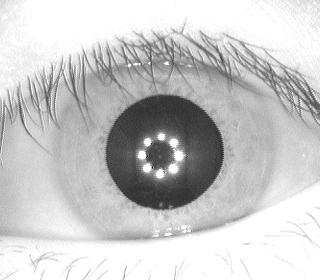
\includegraphics[width=44mm]{tfm-img16}}
\subfigure[S1113R05.jpg]{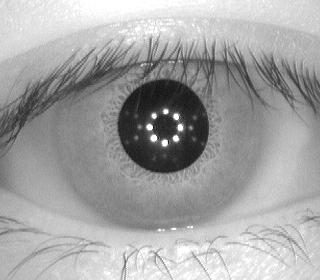
\includegraphics[width=44mm]{tfm-img17}}
\subfigure[S1188L04.jpg]{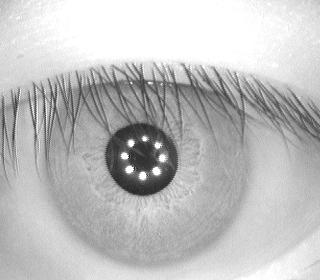
\includegraphics[width=44mm]{tfm-img18}}
\subfigure[S1200R02.jpg]{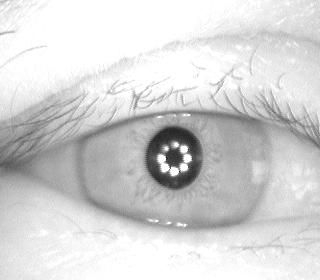
\includegraphics[width=44mm]{tfm-img19}}
\subfigure[S1217L04.jpg]{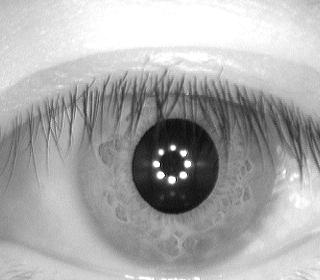
\includegraphics[width=44mm]{tfm-img20}}
\caption{Imágenes de la base de datos CASIA-IrisV4.} \label{fig:señales}
\end{figure}

%----------------------------------------------------------------------------------------

\section{LIP-VIREO}

Es una herramienta multiplataforma para la extracción de características sobre la textura de una imagen basada en puntos de interés locales. Esta desarrollada en C++ y actualmente cuenta con la implementación de ocho detectores de puntos de interés como son \textbf{DoG}, \textbf{LoG}, \textbf{Harris-Laplace}, \textbf{Hessian-Laplace}, \textbf{Harris}, \textbf{Hessian}, \textbf{Fast Hessian} (detector SURF) y \textbf{Dense}. Además cuenta también con un conjunto de descriptores de puntos de interés como \textbf{SIFT}, \textbf{Flip}, \textbf{FIND}, \textbf{PCA-SIFT}, \textbf{SPIN}, \textbf{RIFT}, \textbf{ERIFT}, \textbf{SURF}, \textbf{AoD} y \textbf{LJET}.

Los detectores \textbf{Harris} y \textbf{Harris-Laplace} se basan en diferentes funciones para medir la prominencia de la región alrededor de un pixel. Estos detectores están basados principalmente en la matriz de segundo momento para un punto X como se muetra en la siguiente figura.

\begin{figure}[htbp]
\centering
\[
\mu \left ( X,\sigma _{1},  \sigma _{D}\right ) = \sigma ^{2}_{D}g(\sigma _{I}) * \begin{bmatrix}
L^{2}_{x}(X,\sigma _{D}) \:\:\:\: L_{x}L_{y}(X,\sigma _{D}) \\
L_{x}L_{y}(X,\sigma _{D}) \:\:\:\: L^{2}_{y}(X,\sigma _{D})
\end{bmatrix}
\] 
\caption{Matriz de segundo momento para el detector Harris.} 
\end{figure}

donde $\sigma _{I}$ es la escala de integración, $\sigma _{D}$ es la escala de diferenciación y $L_{g}$ es la derivada calculada en la dirección g (x o y). Esta matriz principalmente describe la distribución del gradiente en un vecindario local de un punto X. \\

A diferencia del detector \textbf{Harris}, la matriz de los detectores \textbf{Hessian} y \textbf{Hessian-Laplace} para un punto dado X viene expresada de la siguiente manera. \\

\begin{figure}[htbp]
\centering
\[
H( X,  \sigma) = 
\begin{bmatrix}
L_{xx}(X,\sigma) \:\:\:\: L_{xy}(X,\sigma) \\
L_{xy}(X,\sigma) \:\:\:\: L_{yy}(X,\sigma)
\end{bmatrix}
\]
\caption{Matriz de segundo momento para el detector Hessian (I).} 
\end{figure}

donde $\sigma$  es el parámetro de suavizado Gaussiano. La ecuación siguiente define la prominencia del punto X solamente basado en el determinante de la matriz Hessian. \\

\begin{figure}[htbp]
\centering
\[
H( X, \sigma _{D} ) = 
\begin{bmatrix}
L_{xx}(X,\sigma_{D}) \:\:\:\: L_{xy}(X,\sigma_{D}) \\
L_{xy}(X,\sigma_{D}) \:\:\:\: L_{yy}(X,\sigma_{D})
\end{bmatrix}
\] 
\caption{Matriz de segundo momento para el detector Hessian (II).} 
\end{figure}

\begin{figure}[htbp]
\centering
\[
Hessian(X, \sigma) = det(H(X,\sigma)) x \sigma^4
\]
\caption{Detector Hessian.} 
\end{figure}

El detector \textbf{Laplaciano de Gauss (LoG)} se basa en la siguiente ecuación para medir la prominencia de un punto X. 

\begin{figure}[htbp]
\centering
\[
LoG(X, \sigma_{I}) = \sigma_{I}(L_{xx}(x,\sigma_{I}) + L_{yy}(x,\sigma_{I}))
\]
\caption{Detector LoG.} 
\end{figure}

Los puntos que alcanzan los máximos locales simultáneamente en sus espacio y escala son los que se seleccionan. Comparando a los detectores vistos anteriormente, podemos observar como en este caso la función de prominencia en el espacio X-Y se ha reemplazado con el laplaciano de Gauss, mientras que la función de prominencia en el espacio de escala se mantiene. Es por eso por lo que estos dos detectores pueden compartir puntos de interés similares. \\

La ecuación de la figura anterior (Figura 3.6) realiza una estimación de las segundas derivadas en las direcciones \textit{x} e \textit{y}, lo que implica que el coste de computación sea relativamente alto. Es por eso por lo que se define una manera más eficiente a través de la \textbf{Diferencia de Gauss DoG} ya que esta solamente requiere la convolución de imágenes de manera constante. \\ \\ \\ \\ \\ \\

\begin{figure}[htbp]
\centering
\[
D(x, y, \sigma) = L(x,y,k\sigma) - L(x,y,\sigma)
\]
\caption{Detector DoG.} 
\end{figure} 

donde $\sigma$ es el parámetro de suavizado Gaussiano y \textit{k} es un multiplicador entero. \\ 

\textbf{Fast Hessian} es el detector de características SURF. Su idea básica es calcular la ecuación de la Figura 3.5 de una manera eficiente con la ayuda de imágenes integrales. Para permitir un cálculo rápido, la ecuación de dicha figura ha sido aproximada de la siguiente manera. 

\begin{figure}[htbp]
\centering
\[
Det(H_{approx}) = D_{xx}D_{yy} - (0.9D_{xy})^2
\]
\caption{Detector Fast Hessian.} 
\end{figure}

donde $D_{xx}$, $D_{yy}$ y $D_{xy}$ son todos calculados eficientemente usando cajas de filtros. \\

\textbf{Dense Sampling} es el último de los detectores de puntos de interés que vamos a ver. Este detector ha mostrado un rendimiento considerablemente mejor que los detectores mejor diseñados en tareas de detección de objetos. El ratio por defecto de este detector es de un punto por cada 10 pixeles. 

%----------------------------------------------------------------------------------------